\chapter{OER in the mobile era: content repositories' features for mobile devices and future trends}


\vfill
Open Contents will have an impact on education in the short term due to the current trend of offering open content for free on the web \citep{TheNewMediaConsortium2010}. Nowadays, a big proportion of the learning materials are accessed form mobile devices. Hence, OER repositories should adapt their capabilities so their contents can be also accessed from mobile devices. This chapter explores common practices in the creation, publication, discovery, acquisition, access, use and re-use of learning objects on mobile devices based on a literature review on research done from 2007 to 2012. From the content providers side, we present the results from a survey performed on 23 educational repository owners prompting them to answer about their current and expected support on mobile devices. From the content user side, we identify features provided by the main OER repositories and relevant apps existing in commercial markets. Finally, we introduce future trends and cues for further research.
\vspace{3em}

This chapter is published as:  Tabuenca, B., Drachsler, H., Ternier, S., \& Specht, M. (2012, December). OER in the Mobile Era: Content Repositories� Features for Mobile Devices and Future Trends. \em Europe elearning papers, Special issue on Mobile learning \em

\clearpage

\section{Introduction}
In 2004 Learning Objects (LOs) have been named in the Horizon report as one of the relevant technology trends \citep{Nmc2004}. This technology appears again in 2010 \cite{TheNewMediaConsortium2010} as open content, predicting to have an impact in the short term due to the current trend of offering open content for free on the Web. 

Open Educational Resources (OERs) not only comprise LOs, course materials, content modules and collections, they also include tools for creating, delivering, using and improving educational contents. \cite{chitwood2002} defined LOs with five characteristics: 1) small units of learning, typically ranging from 2 minutes to 15 minutes; 2)self-contained, each learning object can be taken independently; 3)reusable, a single learning object may be used in multiple contexts for multiple purposes; 4)can be aggregated, learning objects can be grouped into larger collections of content, including traditional course structures; 5)are tagged with metadata, every learning object has descriptive information allowing it to be easily found by a search.
 
The advent of mobile technologies and the boom in 2007 with the birth of smartphones have boosted new ways of interaction. Mobile devices are equipped with capabilities (text editor, audio recorder, video recorder, sensors, internet access, apps, etc.) that facilitate enormously the possibilities to create, publish, discover, acquire, access, use and re-use of educational resources. By mobile device we do not only refer to cell phones, but also to tablets, MP3s, MP4s, game consoles and portable computers. Mobile devices play an important role in lifelong learning. Lifelong learning includes a variety of different educational scenarios and contexts in which learners operate \citep{Tabuenca2013}. Hence, mobile devices facilitate ubiquitous access to OERs stored in content repositories.

In the last years, the usage of mobile devices has grown in many application fields of the education. Likewise, a big proportion of the learning contents are now 'consumed' from mobile devices. OERs are normally stored in open repositories facilitating search, retrieval and re-use among educational communities. The work from \cite{Su2011} summarizes research on adapted mobile content delivery based on mobile capabilities, learners� preferences, and network conditions. 
So far no work was found synthesizing how OER repositories are adapting to mobile learning. Hereby, we extend the research exploring what features are being provided by OER repositories to facilitate access from mobile devices

This chapter is organized as follows. Section two summarizes common practices in the creation, publication, discovery, acquisition, access, use and re-use of learning objects on mobile devices based on a literature review on research trends from 2007 to 2012. The third section presents the results from a survey performed on 23 educational repository owners prompting them to answer about their current and expected support on mobile devices. Section four analyzes the features that the main OER repositories are providing for mobile users. Section five presents discussion and conclusions.
\section{Literature review on learning objects for mobile devices}
This section reviews scientific work on the creation, publication, discovery, acquisition, access, and use of mobile OERs.
\subsection{Method}
Five major digital libraries were selected to find relevant papers in the usage of mobile devices to access OERs repositories: ACM, IEEE, Science Direct, Springerlink and Wiley. We searched the listed libraries constructing search-strings that follow the pattern: all papers published after 2006 that contain (�Mobile� AND �learning� AND �object� AND �repository� AND �content� AND �education�) in their full-text AND (contain (�mobile�) in their keywords OR contain (�mobile�) in the title). 

This query reported the following number of items: 21 in ACM; 165 in IEEE; 26 in ScienceDirect; 36 in Springerlink; 12 in Wiley. For each of these libraries, results were ordered by relevance and the 20 first elements were extracted. The resulting list of 92 papers was manually reviewed. 
\subsection{Results}
\subsubsection{Creation of contents}
Nowadays, mobile devices are equipped with features that facilitate the creation of learning contents. Indeed, most mobile users are capable of recording audios, recording videos or composing a text note. The quality of the audio and video reproducers, and the increase of the size of the screens to display text, has augmented considerably the degree of excellence for consuming contents with respect to the pre-smartphone era. The exploratory study by \cite{Churchill2008} describes considerations to take into account when designing LOs for small-screen handheld devices. 
\subsubsection{Publication of contents}
Standards are being periodically reformulated to adapt the publication of LOs in content repositories. Tagging resources with meta-data is essential to guarantee their reusability. The need for analyzing the issues that raise the inclusion and use of metadata in the learning objects delivered to mobile devices was already pinpointed by \cite{DeMarcos2006} as an investigation line pending to develop. For example, the IEEE LOM specification does not directly support the description of educational resources in terms of their relevance to language learning and mobile-delivery related characteristics as claimed by \citep{Sampson2008}. 

Keeping the standards up-to-date is key for teachers and instructional designers to author, search, acquire, (re)-use and share educational resources effectively.
\subsubsection{Content allocation}
This review has resulted in the following ways to filter contents by context and access it from the mobile device: GPS, compass, Wi-Fi, RFID, infrared, barcode, Bluetooth, text recognition and image recognition. 

\cite{Han2007} used mobile indexed image-recognition to augment real images with an extended multimedia description that was stored in a OER repository. Augmented reality has been also implemented using textbooks  \citep{Santana-mancilla2012}. In this work, secondary school students accessed to additional educational contents related to their textbooks. This system recognizes the images printed in the book as part of regular taught topics and shows multimedia contents that complement the topics covered in the book. Similar, \cite{Chao2009} used markers (printed text identifiers) that can be easily read and tracked by a computer to augment text content with multimedia content.

Excursions of art and museum are good examples of content delivery based on the parameters supplied by mobile devices. Mobile guides delivering contextualized audio, video and text are reviewed in recent work from \cite{Emmanouilidis2013}. This work claims that the current trend is to gradually abandon some of the older localization technologies such as Wi-Fi, infrared and manual user position input. \cite{Oppermann1999c} performed the first relevant experiment using infrared for location identification and wireless LAN for data transmission to and from the server in a museum in which audio contents where delivered from a repository. The near ubiquity of GPS receivers in mobile devices makes this technology extremely popular, nevertheless, they are high battery consumer and they do not work indoors. 

Other localization technologies, such as Radio Frequency IDentification (RFID) and 2D barcodes, have become more popular due to better device support. \citep{Chen2010} implement an augmented reality scenario enriching textbooks with multimedia content stored in a repository. These contents were addressed reading Quick Response (QR) codes printed next to the text to enrich. Similar \cite{Chen2012,Choi2008,Huang2008} present implementations of contextualized content delivery indexed by RFIDs. 

Near Field Communication (NFC) is an extension of RFID technology. RFID is capable of accepting and transmitting beyond a few meters whereas NFC is restricted to four inches. There is a trend  in mobile phones to be equipped with NFC. This type of communication has been evaluated with the aim to access contents stored on OER repositories. A recent experiment implemented a scenario in which a user carrying her mobile phone in a fieldtrip excursion could tap (with her mobile phone) objects augmented with NFC tags. When these tags were by the mobile device, the path to the learning content (i.e. image, video, audio) was decoded and reproduced. Every time a tag was tapped, the action and actor was registered and tracked by the system \citep{Perez-Sanagustin2012}.

\cite{Rahman2011a} implemented a 3D car gaming metaphor to manipulate LOs hosted in repositories, that could be controlled with the gestures identified by the accelerometer of the mobile device (See figure \ref{fig:oerrepos_fig2}). They additionally included a functionality to access, play, and store the learning objects for later browsing through the mobile interface.

\begin{figure}
     \centering
     
\includegraphics[width=0.6\linewidth]{img/oerrepos_fig2}
     \caption{3D car metaphor for navigation between LOs}
     \label{fig:oerrepos_fig2}
\end{figure}

Web browsers keep being the main ways to access LOs  stores in repositories. MERLOT is an example of a portal-based repository adapting the search functionality depending on the type of mobile platform aimed to use the content. \cite{Siadaty} propose the m-LOCO framework for contextualized mobile content delivery, making use of the following repositories: 1) the repository of learning objects includes information about the content format (i.e. audio, video, text) and the educational content types (i.e. exercise, example, overview or tutorial); 2)the delivery media repository contains data about specifications and features of different available delivery media (e.g., mobile devices and PDAs); 3)the context repository is used to perform further analysis or reasoning (e.g., every time a learner selects a learning object from the learning object repository, the related contextual data would be gathered and stored in the repository).

\subsubsection{Standards for content packaging, delivery and sequencing}
IMS Learning Design and the SCORM are the most important interoperability models for reusability in eLearning. This review has identified the following solutions making use of these standards in mobile devices:

\em Pocket-SCORM \em  is a SCORM reader on mobile devices with access to an Learning Management System (LMS) server and a SCORM repository. This tool was first released in June 2004 for Windows Mobile \citep{Chang2005}. To the best our knowledge, the \em Pocket-SCORM\em was not further developed. 

\em SMILE PDA \em  is an open source software implementation for executing IMS Learning Design activities via mobile devices. In contrast to existing IMS Learning Design Players such as Coppercore\footnote{CopperCore, The IMS Learning Design Engine. http://coppercore.sourceforge.net/} and Reload Player\footnote{Reload Project, Reload IMS LD Player. http://www.reload.ac.uk/}, the \em SMILE PDA\em does not need to be connected to the internet during the entire execution time and has been specially designed for delivery through mobile user interfaces as the educational content can be automatically adjusted to the size of the display of the device used \citep{Sampson2008}.

The \em eXact-mobile \em \footnote{eXact mobile http://www.exact-learning.com/en/products/learn-exact-suite/exact-mobile-solution-for-mobile-learning}  is a commercial solution for standard management, delivery and tracking of multimedia for training. This tool features tracking, synching and content authoring according to recognized standards (i.e. SCORM). This tool supports content delivery for Android, iPhone and Blackberry.

The \em PLCAM \em delivers SCORM mobile LOs based on learners� preferences, hardware profile and �satisfaction degree� of these contents in previous usages \citep{Su2011}.
\subsubsection{Architectures framing mobile content delivery}
In the last years, different service-based architectures have been proposed with the aim to provide educational institutions the flexibility to add and re-use services inside the already existing platforms. This way, many basic services and resources do not need to be developed again, reducing considerably the complexity in the design of new educational environments. \cite{MartinProc2009} in their review of existent solutions propose an architecture (figure \ref{fig:oerrepos_fig4}) in which LMS services are transferred to mobile devices from Web-Services that outsource the resources via HTTP.
\begin{figure}
     \centering
     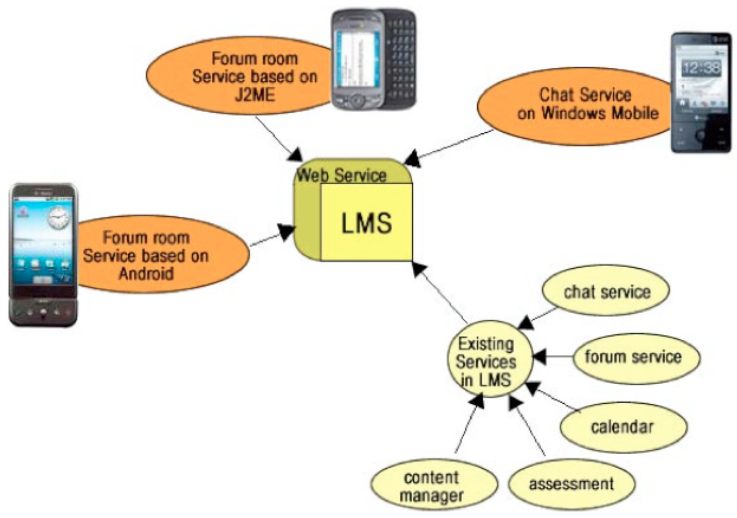
\includegraphics[width=0.6\linewidth]{img/oerrepos_fig4}
     \caption{Integration of LMS services for mobile devices \citep{MartinProc2009}}
     \label{fig:oerrepos_fig4}
\end{figure}
\subsubsection{Content repositories and ubiquitous computing}
Tagging physical objects (books, pictures, sculptures, etc.) with QR codes or RFID tags enriching them with multimedia content has resulted in different implementation in the last years. In most of the cases, the resource repository provide content-related materials that are not originally included in the original physical object. Physical objects can be augmented with texts \citep{Chen2010,Chao2009}, images \citep{Han2007,Santana-mancilla2012} or multimedia \citep{Perez-Sanagustin2012a}. 

This review highlights different examples of ubiquitous computing scenarios broadcasting contextualized learning contents to mobile devices. \cite{Barbosa2007} show how LOs can be delivered to students depending on their physical location and their progress completing a task. More recently, \cite{Rahman2012} designed a prototype that makes use of accelerometer and infrared sensors to distribute and launch LOs to different displays by pointing at them with the mobile device. This approach represents a case of use where the mobile device is used to distribute where contents should be displayed .
\section{A survey to OER repositories on mobile access}
This section presents the results of a survey performed on 23 content repositories, partners of the Open Discovery Space  European project, hosting more than 1,583,000 resources (this is an approximation since some of the contents might be overlapped in more than one repository). The aim of this survey is to gain insights into the way content repositories provide access to mobile devices. Table \ref{tbl:oerrepos_tbl1} lists the repositories participating in the survey.

\begin{table}[h]
  \small
  \caption{Content repositories participating in the survey}
  \label{tbl:oerrepos_tbl1}
\begin{tabular}{lllll}
\thickhline
\textbf{Repository} & \textbf{Scope} & \textbf{\begin{tabular}[c]{@{}c@{}}Num of \\ resources\end{tabular}} & \textbf{} \\ \thickhline
ARIADNE federation           		& International teachers \& students          	& \multicolumn{1}{r}{1,000,000}           &           \\ 
Open Science Resources            	& European science teachers           			& \multicolumn{1}{r}{1,200}           &           \\ 
eduTubeplus library            		& European teachers \& students           		& \multicolumn{1}{r}{5,000}           &           \\ 
COSMOS            					& International science teachers           		& \multicolumn{1}{r}{100,000}           &           \\ 
I2G Intergeo           				& European math teachers \& students           	& \multicolumn{1}{r}{3,500}           &           \\ 
Key2Nature�s Dryades             	& European biology teachers \& students			& \multicolumn{1}{r}{86,000}           &           \\ 
OpenScout federation           		& International teachers \& students           	& \multicolumn{1}{r}{53,000}           &           \\ 
SIVECO�s ASPECT            			& Romanian teachers            					& \multicolumn{1}{r}{1,600}            &           \\ 
FUNecole           					& European teachers \& students            		& \multicolumn{1}{r}{1,500}            &           \\ 
LaProf            					& European language teachers \& students       	& \multicolumn{1}{r}{800}           &           \\ 
Miksike�s LeFo            			& Estonian, Lithuanian \& Latvian teachers     	& \multicolumn{1}{r}{50,000}           &           \\ 
Bulgarian repository           		& Bulgarian teachers \& students           		& \multicolumn{1}{r}{3,500}           &           \\ 
Virtual Bulgaria           			& Bulgarian teachers \& students  				& \multicolumn{1}{r}{7,000}           &           \\ 
Znam.bg            					& Bulgarian teachers \& students           		& \multicolumn{1}{r}{100,000}           &           \\ 
BMU            						& Serbian teachers \& students           		& \multicolumn{1}{r}{180}           &           \\ 
Croatian repository           		& Croatian teachers \& students           		& \multicolumn{1}{r}{2,700}           &           \\ 
Greek repository           			& Greek teachers \& students           			& \multicolumn{1}{r}{1,000}          &           \\ 
Bildung.at          			  	& Austrian teachers           					& \multicolumn{1}{r}{500}           &           \\ 
LMS.at 				           		& Austrian teachers           					& \multicolumn{1}{r}{100,000}           &           \\ 
Ambjorn�s Naeve math           		& Math teachers           						& \multicolumn{1}{r}{300}            &           \\ 
OERCommons.org           			& International teachers           				& \multicolumn{1}{r}{70,000}           &           \\ \hline
\end{tabular}
\end{table}

\subsection{Method}
This survey gathers information about repository�s accessibility via mobile devices, potential future apps and functionalities from the repository owner�s point of view. Content owners received an email in which they were prompted to answer six questions related to mobile usage. Guidelines and examples of possible ways to fill in the requested information were included. The collected files were analyzed obtaining the following results:
\subsection{Results}
Figure \ref{fig:oerrepos_fig7} illustrates the answers reported to the question: Q1.\em Did you prepare your repository to be accessed with different mobile devices?\em . The majority of the repositories (87\%) answered that their repository can be accessed by portable laptops. Tablets are in the second place with 74\% of the repositories. More than 65\% of the repositories are accessible via smartphones. Summarising, more than half of the repositories can be explored by all type mobile devices due to the fact that they were accounting access from a web browser.

\begin{figure}
     \centering
     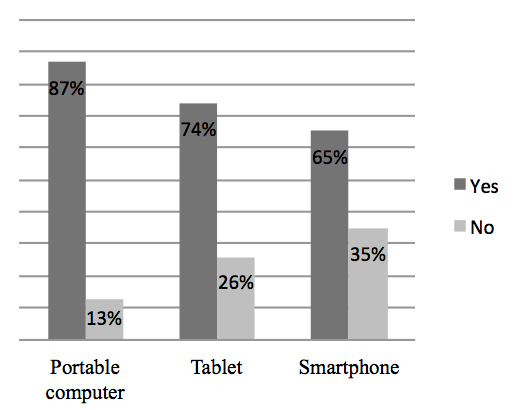
\includegraphics[width=0.5\linewidth]{img/oerrepos_fig7}
     \caption{Question 1: \em Did you prepare your repository to be accessed with different mobile devices?\em. Percentage for n=23 repositories.}
     \label{fig:oerrepos_fig7}
\end{figure}

Contrary to our expectations, the results presented in table \ref{tbl:oerrepos_tbl2} show that the majority of the OER repositories did not consider providing an app to facilitate access from mobile devices. The majority of the owners of the OER repositories reported not knowing a suitable app to facilitate open access from mobile devices. Nevertheless, a big proportion (65\%) of the respondents reported that an app would increase the access rates to their repositories. There is even more consensus in the answers reported to Q5 in which 75\% of the OER repositories indicated that an Application Programming Interface (API) would help them to provide access from different devices.

\begin{table}[h]
  \small
  \caption{Survey to OER repositories}
  \label{tbl:oerrepos_tbl2}
\begin{tabular}{rlrrr}
\thickhline
Q\# & Question                                                                                                                                                                  & Yes  & No   & NA   \\ \thickhline
Q2  & \begin{tabular}[c]{@{}l@{}}Did you consider providing an app to\\ access the content in you repositories?\end{tabular}                                                    & 39\% & 52\% & 9\%  \\
Q3  & \begin{tabular}[c]{@{}l@{}}Do you know any suitable app for accessing\\ content repositories and open content?\end{tabular}                                               & 17\% & 52\% & 30\% \\
Q4  & \begin{tabular}[c]{@{}l@{}}Do you think an app could increase the access\\ rates to your repository?\end{tabular}                                                         & 65\% & 22\% & 13\% \\
Q5  & \begin{tabular}[c]{@{}l@{}}Would you consider providing an application\\ interface (API) to provide access to your\\ repositories from other sites and apps?\end{tabular} & 74\% & 9\%  & 17\% \\ \hline
\end{tabular}
\end{table}

Figure \ref{fig:oerrepos_fig12} illustrates the answers reported to the question: Q6.\em What kind of functionality would be beneficial state of the art access to content repositories? \em Average 60\% of the repositories found ranking of the content, social collaboration, and cloud storage as the most beneficial functionalities to provide mobile access. Furthermore, more than 30\% of the repositories agree that the following functionalities are beneficial to provide state-of-the-art access to content repositories: location-based services, augmented reality, reading voice services, help documentation, version control, schema representing tools to visually link docs and authors, voice-enabled search.

\begin{figure}
     \centering
     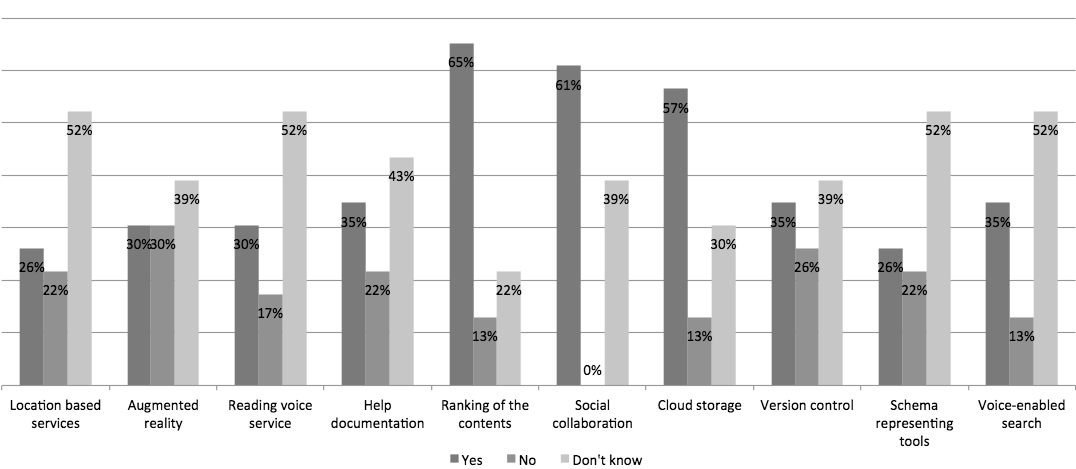
\includegraphics[width=1\linewidth]{img/oerrepos_fig12}
     \caption{Question 6: \em What kind of functionalities would be beneficial to provide state of the art access to content repositories?\em. Percentage for n=23 repositories.}
     \label{fig:oerrepos_fig12}
\end{figure}

\section{OER repositories' features for mobile devices}
This section reviews specific features provided by OER repositories supporting mobile access. Some of the features described here were discovered in the scientific literature review presented in previous sections. Here, we have selected some of the previously cited OER repositories, to describe which initiatives they carried out for mobile support. Additionally, we review relevant referratories that were excluded in the previous section. By referratory we mean repositories that only handle metadata from LOs, while the LOs are stored somewhere in a different repository. The method to analyze them was browsing their sites and exploring the main app markets in Internet (i.e. Google Play, Apple Store).

\begin{figure}
     \centering
     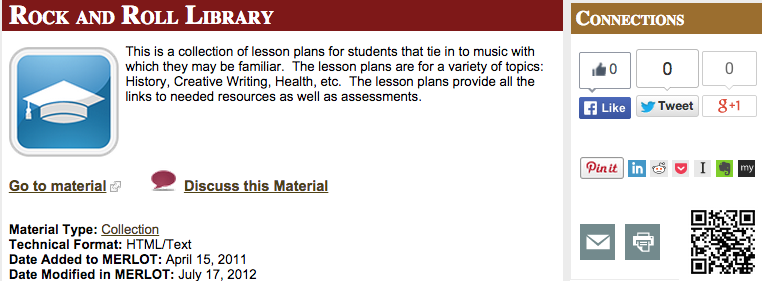
\includegraphics[width=0.9\linewidth]{img/oerrepos_fig15}
     \caption{MERLOT repository. Every LO is listed with a QR codes for augmenting paper material.}
     \label{fig:oerrepos_fig15}
\end{figure}

The \em OpenScout \em  Project was launched in 2012 as a portal that provides free online management of OERs, i.e. search, visualize, use, share and publish. The OpenScout feature an interface to start a keyword-based search, filter search results, include competence search criteria, or add social metadata like tags, comments or ratings. Regarding the features supporting mobile devices, The OpenScout app for iOS provides a keyword search in which the search results are sorted by relevance. The app facilitates access to the details of the resources and bookmark them. Bookmarks are saved locally in the users� device facilitating the organization and collection of items that the user might find relevant.

\em Mobile2Learn \em  is a European Project that aims at improving language-learning instruction by expanding the resources for teaching and learning in vocational education training.  This portal intends to promote access to mobile-supported training services for the provision of on-demand lifelong language learning beyond time and place restrictions. Mobile2Learn provides a stand-alone application (MW-TELL) that can be installed in a PDA or smartphone device and facilitates the delivery of mobile training courses. The main functionalities of MW-TELL Courses PDA include: delivery of mobile training courses packages for English language learning; support of multiples roles, such as individual learners and tutors; rendering of HTML�based content and flash files conformant with the IMS Learning Design (v1.0 Level A specification) and IMS Content Packaging (v1.1.4 specification).  \cite{Sampson2012} present an implementation of the Mobile2Learn framework for English language-learning concluding the following indications: existing Mobile-Assisted Lifelong Language Learning (MALL) resources can be re-used within different MALL courses, while retaining their open access by different platforms and systems; existing MALL course templates can be re-used within different MALL courses addressing teaching of a specific language. The features from MW-TELL are further described in \citep{Romero}.
 	 	 
\em MERLOT \em  is a free and open online community of resources designed primarily for faculty, staff and students of higher education around the world to share their learning materials and pedagogy. MERLOT provides different capabilities for mobile support. The free MERLOT OER search app for iOS and Android-based mobile devices searches the MERLOT database for open educational materials. MERLOT OER dearch app enables mobile users to retrieve detailed, discipline-based information on thousands of open courses, open texts, and open journal articles directly from MERLOT�s internationally renowned digital library.  Retrieved information includes all the comments, ratings, related learning exercises, and peer review information, with links directly to the learning materials in the hit list. It is possible to share findings with colleagues via mobile device. All the materials listed in MERLOT include a QR code with an URL redirecting to the learning materials so they can be easily shared or bound to paper materials (See figure \ref{fig:oerrepos_fig15}). Additionally, MERLOT provides an advanced search for materials designed for mobile devices including the criteria �Type of delivery platform� to the information (metadata on smartphones, tablets, LMS�s). 

\begin{figure}
     \centering
     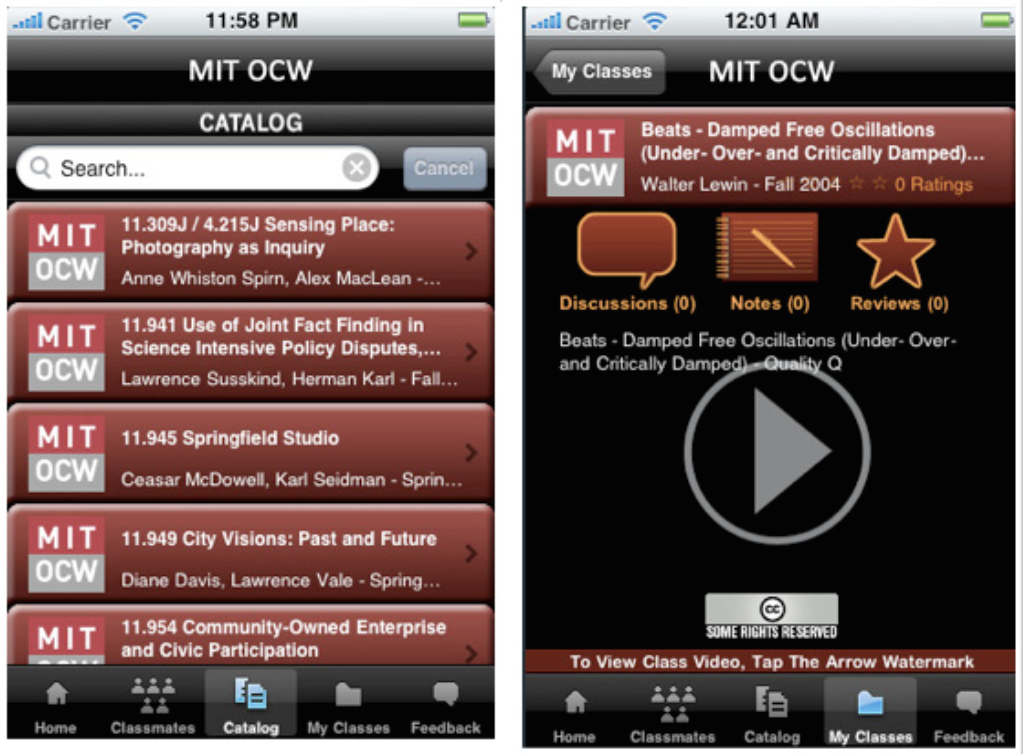
\includegraphics[width=0.6\linewidth]{img/oerrepos_fig16}
     \caption{iOS app for MIT OpenCourseWare}
     \label{fig:oerrepos_fig16}
\end{figure}

\em The OpenCourseWare (OCW) \em movement initially started in T�bingen (Germany), was finally launched at Massachusetts Institute of Technology (OCW-MIT), an open, free, web-based publication of all courses and contents taught at MIT. This initiative has been widely extended to multiple universities around the world. MIT-OCW released their iPhone app in February 2011 (figure \ref{fig:oerrepos_fig16}) allowing to access OCW videos stored in iTunes. Its social learning experience makes this app different from others. This app includes a virtual space called �classmates� where students can discuss with colleagues. 

\em Khan Academy�s \em website supplies a free online collection of more than 3,500 micro lectures via video tutorials stored on YouTube covering a broad range of educational topics. Khan Academy has a higher rate of videos viewed in comparison to MIT's OCW . The Kahn Academy launched an official app both for Android and iPhone (figure \ref{fig:oerrepos_fig17}) and iPad app (March 2012). Its main functionality is providing access to videos. There are also unofficial viewer apps that let import the Facebook profile (figure \ref{fig:oerrepos_fig17} right).

\begin{figure}
     \centering
     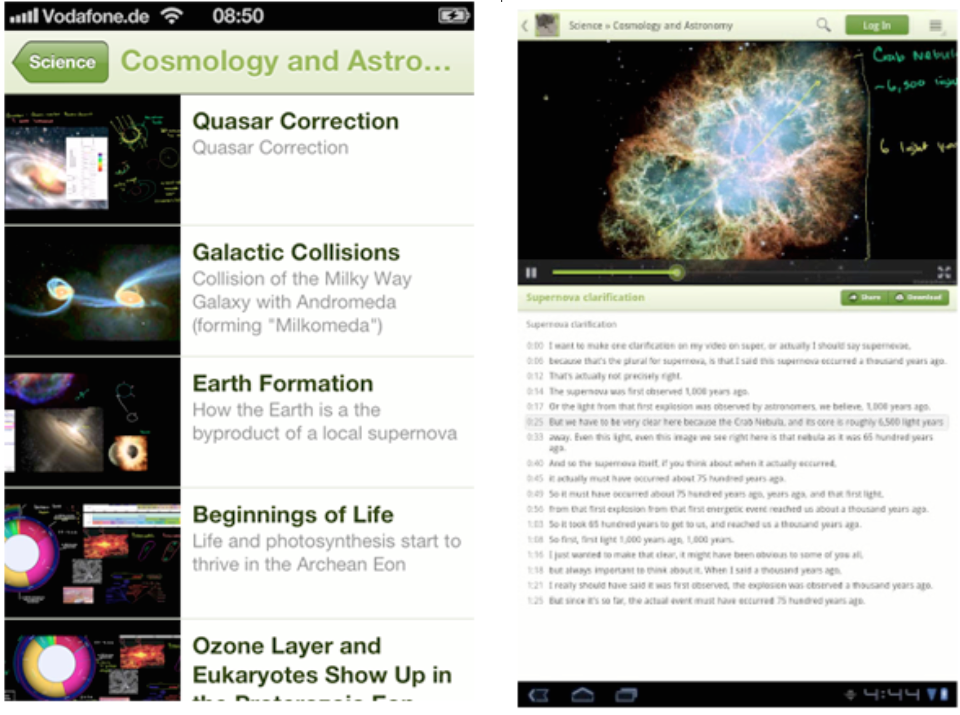
\includegraphics[width=0.6\linewidth]{img/oerrepos_fig17}
     \caption{Mobile apps for visualising videos from Khan Academy. iOS official app on the left. Android unofficial app on the right.}
     \label{fig:oerrepos_fig17}
\end{figure}

\section{Discussion and conclusions}
Mobile devices facilitate new ways to access content from OER repositories. This chapter has shed light on different prototypes and tools using GPS, compass, Wi-Fi, RFID, NFC, infrared, QR code, Bluetooth, text recognition, image recognition or the accelerometer to index contents stored in OER repositories. These prototypes have been tested in different learning contexts \citep{Chen2010,Chao2009,Han2007,Santana-mancilla2012,Perez-Sanagustin2012a,Barbosa2007,Rahman2012}. This study shows cues on how to augment physical objects (books, museums, etc.) with digital learning contents delivered to mobile devices and extracted from content repositories.

Easy to create and consume mobile contents are those whose unit of construction (granularity) is less complex, i.e. text, audio or video. Nowadays, smartphones and tablets are equipped from scratch with tools that facilitate easy creation and consumption of this type of materials, as no special app or feature needs to be installed. Most of the studies reviewed in this chapter pull materials with low granularity. The work from \cite{Yang2007} adapting already existing desktop-based learning materials to the mobile setting advise the use of technologies like HTML5 to make easier integration of audio, video, and texts in mobile platforms (see Khan Academy official app). Adapting more complex contents like LOs to mobile LOs is hard to sustain in long terms since mobile technology is continuously evolving the features from new mobile devices. Previous LOs were designed and created for desktop platforms and some of their features are missed when moved to a mobile context (screen size, content sequencing, etc.). \cite{Bradley2009} describe this incompatibility as follows: � \em LOs were developed to tackle a series of pedagogical challenges, such as facilitating learner engagement, and aiding students in dealing with problems of abstraction and complexity. These learning objects use a number of constructivist principles provided by rich interactive visualizations or learner controlled pacing \em �. The review of the apps existing in commercial market concluded with no �killer app� adapting desktop-based LOs to for mobile devices. We have highlighted apps sequencing learning contents (e.g. eXact and MW-TELL mobile app), as well as best practices to scaffold architectures to facilitate across platform accessibility (iOS, Android, Windows) compatibility like web-services, APIs, or HTML5.

From the repository� point of view, the results of the survey indicate that the majority of the content repositories are accessible by different mobile devices (via web browser). These results provide an overall view of the extent to which repositories are in a significant need to adapt their architectures for mobile devices rather than adapting the content. Hence, repositories should provide content that can be delivered via HTTP (e.g. via web-services) to any device, as well as following formatting (e.g. HTML5) and sequencing (e.g. SCORM) standards to foster universal access to open communities.
